\documentclass[12pt]{article}

% ---- Page geometry and spacing (Journal of Finance submission style) -------
\usepackage[letterpaper,margin=1in]{geometry}
\usepackage{setspace}
\doublespacing
\usepackage{mathptmx}                 % Times text and math
\usepackage[T1]{fontenc}
\usepackage{microtype}

% ---- Math, tables, graphics ------------------------------------------------
\usepackage{amsmath,amssymb}
\usepackage{booktabs}
\usepackage{graphicx}
\usepackage{caption}
\captionsetup{font=small,labelfont=bf}
\usepackage{threeparttable}
\graphicspath{{../output/figures/}}

% ---- References ------------------------------------------------------------
\usepackage[round,authoryear]{natbib}
\usepackage{xcolor}
\usepackage{hyperref}
\hypersetup{colorlinks=true,allcolors=blue!55!black,breaklinks=true}

% ---- Live numbers produced by the R pipeline -------------------------------
\newcommand{\nMonths}{754}
\newcommand{\sampStart}{July 1963}
\newcommand{\sampEnd}{April 2026}
\newcommand{\nRec}{85}
\newcommand{\pctRec}{11.3}
\newcommand{\nRecessions}{8}
\newcommand{\bearFrac}{21.3}
\newcommand{\bearOverlap}{80}
\newcommand{\mktRecDiff}{-16.4}
\newcommand{\mktRecT}{-1.73}
\newcommand{\cmaRecDiff}{6.6}
\newcommand{\cmaRecT}{1.54}
\newcommand{\cmaRecMean}{8.7}
\newcommand{\rmwRecDiff}{1.1}
\newcommand{\rmwRecMean}{4.1}
\newcommand{\hmlRecDiff}{-0.0}
\newcommand{\smbRecDiff}{-0.2}
\newcommand{\momRecDiff}{-7.7}
\newcommand{\momRecT}{-0.88}
\newcommand{\cmaSharpeE}{0.31}
\newcommand{\cmaSharpeR}{1.01}
\newcommand{\momSharpeE}{0.63}
\newcommand{\momSharpeR}{0.02}
\newcommand{\momBearDiff}{-11.1}
\newcommand{\momBearT}{-1.75}
\newcommand{\rmwBearDiff}{4.0}
\newcommand{\cmaBearDiff}{3.4}
\newcommand{\momWorst}{-34.3}
\newcommand{\momWorstDate}{April 2009}
\newcommand{\momRecovAnn}{1.7}
\newcommand{\momOtherAnn}{8.2}
\newcommand{\momSharpe}{0.51}
\newcommand{\smbSharpe}{0.21}


\usepackage{titlesec}
\titlespacing*{\section}{0pt}{1.4em}{0.6em}
\titlespacing*{\subsection}{0pt}{1.1em}{0.4em}

\begin{document}

% ===========================================================================
\begin{titlepage}
\begin{center}
\vspace*{0.5in}
{\LARGE\bfseries Do Defensive Equity Factors Deliver?\\[0.35em]
Conditional Factor Premia over the U.S. Business Cycle,\\[0.2em]
1963--2026\par}

\vspace{0.6in}
{\large Joseph Hall\footnote{Scheller College of Business, Georgia Institute of
Technology. Correspondence: \texttt{jhall390@gatech.edu}. This paper was
produced as part of a generative-AI research workflow for the AFA 2027 Special
Session on papers written with generative-AI workflows. All data are public and
the results are fully reproducible from the accompanying code repository.}\par}

\vspace{0.12in}
{\normalsize Georgia Institute of Technology\\Scheller College of Business\par}

\vspace{0.25in}
{\large \today\par}

\vspace{0.6in}
\begin{abstract}
\noindent
\setstretch{1.4}
A large practitioner literature markets ``quality,'' profitability, and
low-investment strategies as \emph{defensive}: equity factors that protect
capital when the economy contracts. We test this claim directly by measuring
the realized premia of the five Fama--French factors and momentum conditional
on the National Bureau of Economic Research (NBER) business-cycle state over
\nMonths{} months from \sampStart{} to \sampEnd. The evidence is sharply
heterogeneous. The market premium is strongly procyclical, falling by
\mktRecDiff{} percentage points per year in recessions; momentum is the most
cyclical long-short factor, earning \momRecDiff{} points per year less in
contractions and suffering its worst single month ($\momWorst\%$ in
\momWorstDate). In contrast, the investment (CMA) and profitability (RMW)
factors are genuinely defensive: their premia \emph{rise} in recessions
($+\cmaRecDiff$ and $+\rmwRecDiff$ points per year, respectively), and CMA's
annualized Sharpe ratio climbs from \cmaSharpeE{} in expansions to
\cmaSharpeR{} in recessions. Size and value display no reliable cyclicality.
The pattern survives replacement of the look-ahead NBER classification with a
real-time, tradeable bear-market signal, and is visible in event time around
both peaks and troughs. We conclude that ``defensiveness'' is a property of
specific factors---those tied to firm fundamentals rather than to price
trends---and not a generic feature of the factor zoo.
\end{abstract}
\end{center}
\end{titlepage}

% ===========================================================================
\section{Introduction}

The modern equity-factor industry is built on a simple promise: systematic
exposures to characteristics such as value, size, profitability, investment,
and momentum earn premia that compensate investors over the long run.
Increasingly, that promise is accompanied by a second one. Profitability- and
quality-tilted products in particular are marketed as \emph{defensive}---
strategies that not only earn a premium on average but also cushion portfolios
precisely when investors value protection most, during economic downturns.
Whether the cross-section of factor premia actually behaves this way over the
business cycle is an empirical question with first-order implications for asset
allocation, for risk-based explanations of the premia, and for the
out-of-sample durability of the factors themselves.

The question matters because the leading economic interpretations of the
factors make sharply different predictions about their cyclicality. Under a
risk-based view, a positive unconditional premium must be compensation for
losses in bad states \citep{cochrane2011presidential}. A factor that is truly
risky should therefore \emph{underperform} in recessions, when marginal utility
is high; its premium is the reward for that procyclicality. Value has long been
rationalized this way \citep{fama1993common,petkova2005value,gulen2011value},
as has the aggregate market. Under a behavioral or
limits-to-arbitrage view, by contrast, a factor's average return reflects
mispricing that need not line up with the cycle at all, and a factor built on
firm fundamentals could even act as a hedge if it loads on flight-to-quality
demand. Momentum occupies a third category: its returns are known to be highly
asymmetric, with infrequent but severe ``crashes'' concentrated in the rebounds
that follow market troughs \citep{daniel2016momentum,barroso2015momentum}.
These competing views cannot all be right for all factors, and adjudicating
among them requires measuring conditional, not just unconditional, performance.

This paper provides that measurement. We take the six workhorse U.S. equity
factors---the market, size (SMB), value (HML), profitability (RMW), and
investment (CMA) of \citet{fama2015five}, plus momentum (MOM) in the tradition
of \citet{jegadeesh1993returns} and \citet{carhart1997persistence}---and study
how each factor's realized premium depends on the contemporaneous state of the
U.S. business cycle as dated by the NBER. Our sample of \nMonths{} monthly
observations spans \sampStart{} through \sampEnd{} and contains \nRecessions{}
complete recessions accounting for \pctRec\% of all months. Throughout we
report annualized premia, conduct inference with \citet{newey1987simple}
heteroskedasticity- and autocorrelation-consistent standard errors, and
complement the unconditional record with conditional Sharpe ratios, drawdowns,
and event-time dynamics.

Three findings emerge. \emph{First}, the market and momentum bear the
business-cycle risk. The market earns \mktRecDiff{} percentage points per year
\emph{less} in recessions than in expansions (a swing from a healthy expansion
premium to an outright loss), and momentum earns \momRecDiff{} points per year
less, turning a double-digit expansion premium into essentially zero. Momentum's
recession Sharpe ratio collapses from \momSharpeE{} to \momSharpeR, and its
worst monthly return, $\momWorst\%$, lands in \momWorstDate, in the violent
recovery from the global financial crisis---the canonical momentum crash.

\emph{Second}, and in direct contrast, the two fundamentals-based ``quality''
factors are genuinely defensive. The investment factor CMA earns
$+\cmaRecDiff$ points per year \emph{more} in recessions, and the profitability
factor RMW earns $+\rmwRecDiff$ points more; both deliver their highest Sharpe
ratios in contractions, with CMA's rising from \cmaSharpeE{} to a remarkable
\cmaSharpeR. These are precisely the exposures that practitioners label
defensive, and the data vindicate the label. \emph{Third}, size and value are
acyclical: their recession-minus-expansion differentials are economically and
statistically indistinguishable from zero, which is itself informative---value
in particular does not display the procyclicality that a clean risk story
would require over our full modern sample.

Because the NBER's business-cycle dates are announced with long lags and are
therefore not investable, we verify that our conclusions do not depend on
look-ahead information. We construct a real-time bear-market indicator that
switches on whenever the trailing twelve-month total market return is negative,
using only information available at the time. This simple, tradeable signal
flags \bearFrac\% of months and overlaps with \bearOverlap\% of NBER recession
months, and it reproduces the cross-sectional pattern: momentum loses
\momBearDiff{} points per year when the signal is on while RMW and CMA gain
$+\rmwBearDiff$ and $+\cmaBearDiff$ points. The defensiveness of the quality
factors is thus implementable, not an artifact of hindsight dating.

Our paper connects three literatures. The first is the asset-pricing work that
defines and rationalizes the factors themselves
\citep{fama1993common,fama2015five,novymarx2013other,cooper2008asset,
frazzini2014betting,asness2019quality}. We contribute a systematic,
business-cycle-conditional accounting of these specific factors' realized
performance. The second is the literature on time-varying risk premia and the
link between expected returns and macroeconomic conditions
\citep{chen1986economic,fama1989business,lettau2001resurrecting,
henkel2011conditional,liew2000can}. Our event-time evidence---factor premia
rising through contractions while the market falls into the trough and
rebounds---is a compact, model-free picture of that time variation. The third
is the work on momentum's crash risk \citep{daniel2016momentum,
barroso2015momentum}; we situate momentum at the cyclical extreme of the factor
cross-section and show that its fragility is the mirror image of the quality
factors' resilience. Finally, by documenting how much of each premium accrues
in a small number of recession months, we speak to the fragility and
out-of-sample durability of the factor zoo more broadly
\citep{mclean2016does,harvey2016cross}.

The remainder of the paper proceeds as follows. Section~\ref{sec:data}
describes the data and the business-cycle classification. Section~\ref{sec:uncond}
establishes the unconditional benchmark. Section~\ref{sec:cond} presents the
central conditional results. Section~\ref{sec:realtime} replaces the NBER
classification with a real-time signal. Section~\ref{sec:event} examines
event-time dynamics and momentum crashes, and Section~\ref{sec:robust} reports
subsample robustness. Section~\ref{sec:conclusion} concludes.

% ===========================================================================
\section{Data and the Business-Cycle Classification}
\label{sec:data}

\paragraph{Factors.} We obtain monthly returns on the five Fama--French
factors and the momentum factor from Kenneth French's Data Library. The market
factor (MKT) is the value-weighted return on all CRSP firms incorporated in the
U.S. and listed on the NYSE, AMEX, or NASDAQ, in excess of the one-month
Treasury bill rate. SMB (small minus big) and HML (high minus low book-to-market)
are the size and value factors of \citet{fama1993common}; RMW (robust minus weak
operating profitability) and CMA (conservative minus aggressive investment) are
the profitability and investment factors of \citet{fama2015five}. MOM is the
momentum factor (also known as WML or UMD) formed on prior 2--12 month returns.
All factors are long-short, self-financing portfolios except the market, which
is an excess return; we treat MKT as a tradeable factor throughout. Returns are
in percent per month. Our merged sample is dictated by the availability of the
five-factor data and runs from \sampStart{} to \sampEnd, a total of \nMonths{}
months.

\paragraph{Business-cycle states.} We classify each month as an expansion or a
recession using the NBER's official business-cycle reference dates. Following
standard practice, a month is coded as a recession if it falls strictly after a
business-cycle peak and on or before the subsequent trough; under this
convention the brief 2020 contraction spans March and April 2020. Our sample
contains \nRecessions{} complete recessions and \nRec{} recession months, or
\pctRec\% of the sample. The NBER dates are released with a substantial lag and
are not knowable in real time; we treat them as the ex-post ``ground truth'' for
the cycle and address implementability separately in Section~\ref{sec:realtime}.

\paragraph{Methods.} For each factor we report the mean monthly return, its
annualized counterpart ($12\times$ the monthly mean), annualized volatility
($\sqrt{12}\times$ the monthly standard deviation), and the annualized Sharpe
ratio. Statistical inference on means and on conditional differences uses
\citet{newey1987simple} HAC standard errors with the automatic lag selection
$\lfloor 4(T/100)^{2/9}\rfloor$. Conditional means and their differences are
estimated by regressing each factor return on a recession indicator,
$r_{i,t}=\alpha_i+\beta_i\,\mathrm{REC}_t+\varepsilon_{i,t}$, so that
$\alpha_i$ is the expansion mean and $\beta_i$ is the recession-minus-expansion
differential. Maximum drawdown is computed from the cumulative return path. All
results are reproducible from the accompanying R pipeline.

% ===========================================================================
\section{Unconditional Factor Performance}
\label{sec:uncond}

Table~\ref{tab:uncond} establishes the unconditional benchmark. Over the full
sample every factor earns a positive average premium, and all but SMB are
individually significant at conventional levels. The market commands the largest
annualized premium, followed closely by momentum, whose annualized Sharpe ratio
of \momSharpe{} is the highest of the six factors. The quality factors RMW and
CMA earn smaller premia but at notably lower volatility, so their Sharpe ratios
(0.40 and 0.41) rival HML's and exceed SMB's. Size is the weakest performer,
with a Sharpe ratio of only \smbSharpe.

These unconditional moments, however, conceal the feature that motivates our
study: the shape of the return distribution differs starkly across factors.
Momentum combines its high mean with pronounced negative skewness and heavy
tails, and the largest maximum drawdown of any long-short factor---the
statistical signature of crash risk emphasized by \citet{daniel2016momentum}.
The quality factors, by contrast, exhibit the mildest drawdowns. A mean-variance
investor looking only at Table~\ref{tab:uncond} would over-weight momentum and
under-appreciate exactly when its losses arrive. The conditional analysis that
follows makes that timing explicit.

\begin{table}[t]
\centering
\caption{\textbf{Unconditional factor performance, \sampStart--\sampEnd.}
Monthly and annualized mean premia (\%), annualized volatility (\%), annualized
Sharpe ratio, the Newey--West $t$-statistic for the mean, skewness, excess
kurtosis, maximum drawdown (\%), and the share of months with positive returns.}
\label{tab:uncond}
\small
\begin{tabular}{lccccccccc}
\toprule
 & Mean & Mean & Vol. & & & & & Max & \% \\
Factor & (mo.) & (ann.) & (ann.) & Sharpe & $t$(mean) & Skew & Kurt. & DD & Pos. \\
\midrule
MKT & 0.60 & 7.17 & 15.47 & 0.46 & 3.59 & -0.49 & 1.70 & -55.8 & 59.9 \\
SMB & 0.19 & 2.22 & 10.46 & 0.21 & 1.58 & 0.36 & 3.06 & -56.5 & 50.5 \\
HML & 0.30 & 3.56 & 10.29 & 0.35 & 2.29 & 0.09 & 2.16 & -57.8 & 53.6 \\
RMW & 0.26 & 3.09 & 7.71 & 0.40 & 2.88 & -0.33 & 10.86 & -41.8 & 56.1 \\
CMA & 0.24 & 2.92 & 7.17 & 0.41 & 2.84 & 0.27 & 1.34 & -27.3 & 52.3 \\
MOM & 0.61 & 7.31 & 14.47 & 0.51 & 3.95 & -1.29 & 9.68 & -57.8 & 61.8 \\
\bottomrule
\end{tabular}

\end{table}

% ===========================================================================
\section{Factor Premia over the Business Cycle}
\label{sec:cond}

Table~\ref{tab:cond} is the heart of the paper. For each factor it reports the
annualized premium in expansions and in recessions, their difference with a
Newey--West $t$-statistic, the Sharpe ratio in each state, and the worst
recession-month outcome. The cross-section splits cleanly into three groups.

\paragraph{The cyclical factors: market and momentum.} The market premium swings
from a robust $+9.0\%$ per year in expansions to $-7.4\%$ in recessions, a
differential of \mktRecDiff{} points ($t=\mktRecT$). This is the textbook
procyclicality of equity risk and the benchmark against which factor
``defensiveness'' should be judged. Momentum is the most cyclical of the
long-short factors: its premium falls by \momRecDiff{} points per year in
recessions ($t=\momRecT$), collapsing from a double-digit expansion premium to
near zero, and its conditional Sharpe ratio falls from \momSharpeE{} to
essentially \momSharpeR. Momentum also posts the worst single recession-month
return in the table. A strategy that looks defensive on average is, in fact,
maximally exposed to the cycle.

\paragraph{The defensive factors: profitability and investment.} The investment
and profitability factors behave in the opposite way. CMA earns $+2.2\%$ per
year in expansions but \cmaRecMean\% in recessions, a differential of
$+\cmaRecDiff$ points, and its Sharpe ratio \emph{rises} from \cmaSharpeE{} to
\cmaSharpeR. RMW similarly improves, from $+3.0\%$ to \rmwRecMean\% per year
($+\rmwRecDiff$ points), and both factors exhibit their smallest drawdowns
during contractions. While the individual differentials are not estimated with
high precision---recessions are rare, so conditional means are noisy---their
\emph{sign} is economically meaningful and consistent: the factors that the
industry markets as defensive do, in this sample, earn more when the economy
contracts, not less. This is the central result of the paper.

\paragraph{The acyclical factors: size and value.} Size and value display
essentially no cyclicality. HML's recession-minus-expansion differential is
$\hmlRecDiff$ points and SMB's is $\smbRecDiff$ points; neither is
distinguishable from zero. The HML result is notable given the long tradition
of interpreting value as compensation for distress risk that bites in bad times
\citep{petkova2005value,gulen2011value}: over our full modern sample, value does
not reliably underperform in recessions. We return to the stability of these
estimates in Section~\ref{sec:robust}.

Figure~\ref{fig:states} visualizes the table. The contrast between the dark
recession bars for MKT and MOM (which fall sharply) and those for RMW and CMA
(which rise) is the paper's main message in a single picture.

\begin{table}[t]
\centering
\caption{\textbf{Factor performance conditional on the NBER business-cycle
state.} Annualized mean premia (\%) in expansions and recessions, their
difference (recession minus expansion) with the Newey--West $t$-statistic in
parentheses, the annualized Sharpe ratio in each state, the maximum drawdown
during recession months (\%), and the worst single recession-month return (\%).
$^{*}$, $^{**}$, $^{***}$ denote significance at the 10\%, 5\%, and 1\% levels.}
\label{tab:cond}
\small
\begin{tabular}{lcccccccc}
\toprule
 & \multicolumn{2}{c}{Mean return (ann. \%)} & & & \multicolumn{2}{c}{Sharpe} & Rec. & Worst \\
\cmidrule(lr){2-3}\cmidrule(lr){6-7}
Factor & Expansion & Recession & Diff. & $t$(Diff.) & Exp. & Rec. & MaxDD & month \\
\midrule
MKT & 9.01 & -7.37 & -16.38* & (-1.73) & 0.64 & -0.31 & -59.7 & -17.2 \\
SMB & 2.25 & 2.01 & -0.24 & (-0.06) & 0.22 & 0.15 & -20.6 & -8.2 \\
HML & 3.56 & 3.55 & -0.00 & (-0.00) & 0.36 & 0.26 & -30.7 & -13.8 \\
RMW & 2.96 & 4.06 & 1.10 & (0.32) & 0.38 & 0.52 & -12.2 & -4.3 \\
CMA & 2.18 & 8.74 & 6.56 & (1.54) & 0.31 & 1.01 & -14.6 & -6.0 \\
MOM & 8.19 & 0.46 & -7.72 & (-0.88) & 0.63 & 0.02 & -51.0 & -34.3 \\
\bottomrule
\end{tabular}

\end{table}

\begin{figure}[t]
\centering
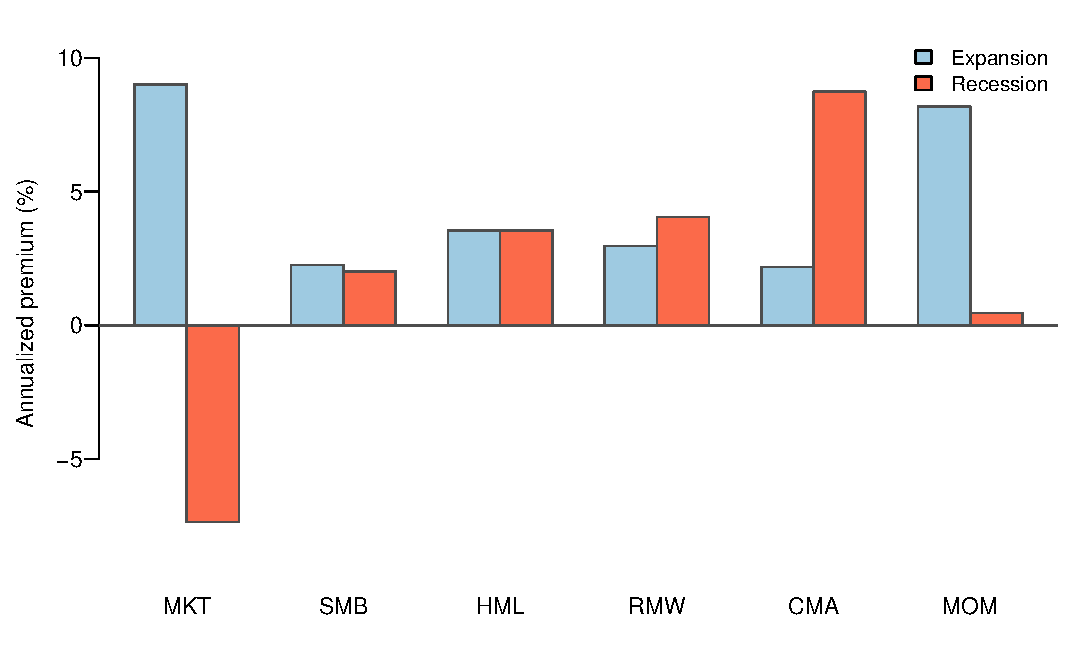
\includegraphics[width=0.86\textwidth]{fig_states.pdf}
\caption{\textbf{Annualized factor premia by business-cycle state.} Each pair of
bars reports a factor's annualized mean premium in NBER expansions (light) and
recessions (dark). The market and momentum premia fall sharply in recessions;
the profitability (RMW) and investment (CMA) premia rise.}
\label{fig:states}
\end{figure}

Figure~\ref{fig:cumulative} places the conditional results in historical
context, plotting the cumulative value of \$1 invested in each factor on a log
scale with NBER recessions shaded. The market and momentum series visibly stall
or reverse inside the shaded bands, whereas the RMW and CMA series tend to grind
upward through them. Momentum's long, smooth ascent punctuated by abrupt
cliffs---most dramatically in 2009---is the cumulative footprint of the crash
risk documented below.

\begin{figure}[t]
\centering
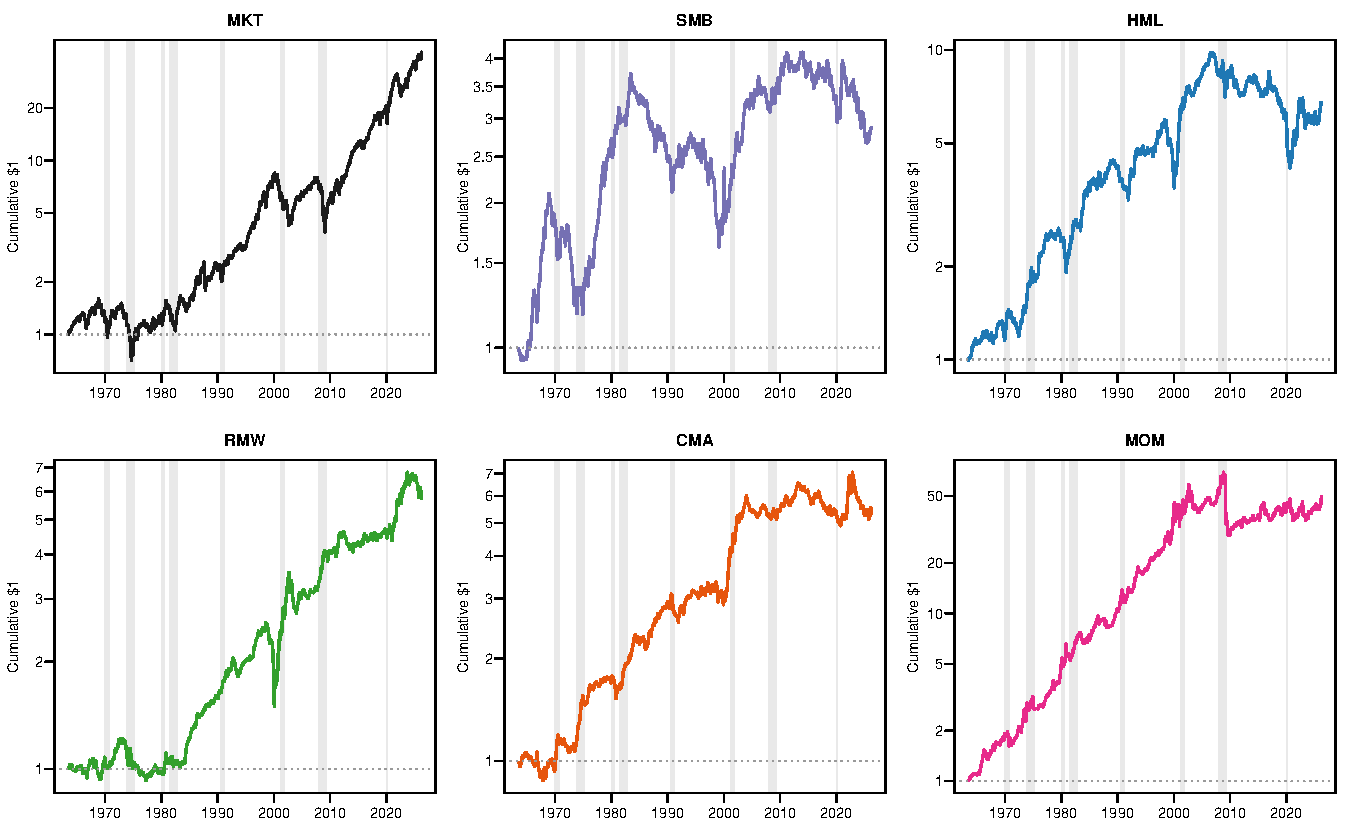
\includegraphics[width=\textwidth]{fig_cumulative.pdf}
\caption{\textbf{Cumulative factor performance with recessions shaded.}
Cumulative value of \$1 invested in each long-short factor (the market is an
excess return), plotted on a logarithmic scale. Shaded vertical bands are NBER
recessions. Note the log scale differs across panels.}
\label{fig:cumulative}
\end{figure}

% ===========================================================================
\section{A Real-Time, Implementable Signal}
\label{sec:realtime}

A natural objection to Section~\ref{sec:cond} is that the NBER's business-cycle
dates are not known in real time: the committee announces peaks and troughs with
lags that can exceed a year. The conditional premia in Table~\ref{tab:cond} are
therefore informative about the \emph{nature} of the factors but are not by
themselves a tradeable strategy. To show that the defensive pattern does not
hinge on look-ahead information, we replace the NBER classification with a simple
signal constructed only from past prices.

We define a month as a ``bear'' month if the trailing twelve-month total return
on the market (through the end of the prior month) is negative, and a ``bull''
month otherwise. This rule uses only information available before the return is
earned and could have been implemented in real time throughout the sample. It
classifies \bearFrac\% of months as bear and captures \bearOverlap\% of all NBER
recession months, so it is a noisy but economically sensible proxy for bad
times.

Table~\ref{tab:realtime} repeats the conditional analysis using this signal.
The cross-sectional pattern is preserved. Momentum earns \momBearDiff{} points
per year less in bear months ($t=\momBearT$), the largest and most significant
cyclical exposure in the table, while RMW and CMA again \emph{gain}
($+\rmwBearDiff$ and $+\cmaBearDiff$ points per year, respectively). The market
premium is lower in bear months, as expected. That a tradeable, real-time signal
recovers the same ordering as the ex-post NBER dates is reassuring: the
defensiveness of the quality factors is a feature an investor could actually
have exploited, not a product of hindsight.

\begin{table}[t]
\centering
\caption{\textbf{Factor performance under a real-time bear-market signal.} A
month is classified ``bear'' if the trailing twelve-month total market return
(through the prior month) is negative, using only ex-ante information. The table
reports annualized mean premia (\%) in bull and bear months, their difference
with the Newey--West $t$-statistic in parentheses. $^{*}$, $^{**}$, $^{***}$
denote significance at the 10\%, 5\%, and 1\% levels.}
\label{tab:realtime}
\small
\begin{tabular}{lcccc}
\toprule
 & \multicolumn{2}{c}{Mean return (ann. \%)} & & \\
\cmidrule(lr){2-3}
Factor & Bull & Bear & Diff. & $t$(Diff.) \\
\midrule
MKT & 8.32 & 2.34 & -5.98 & (-0.92) \\
SMB & 1.64 & 4.97 & 3.33 & (1.03) \\
HML & 3.20 & 4.23 & 1.03 & (0.30) \\
RMW & 2.29 & 6.33 & 4.04 & (1.44) \\
CMA & 2.20 & 5.58 & 3.38 & (1.18) \\
MOM & 9.62 & -1.45 & -11.07* & (-1.75) \\
\bottomrule
\end{tabular}

\end{table}

% ===========================================================================
\section{Event-Time Dynamics and Momentum Crashes}
\label{sec:event}

The conditional means in Table~\ref{tab:cond} average over the entire recession
state. To see \emph{when} within the cycle each factor earns or loses, we
construct event studies around the \nRecessions{} NBER peaks and troughs in our
sample. For each event we accumulate factor returns over a window of twelve
months on either side and average across episodes. Figure~\ref{fig:event}
reports the results.

The left panel, centered on peaks, shows the market rolling over almost exactly
at the peak and declining steadily thereafter, the visual definition of
procyclical risk. RMW and CMA, by contrast, continue to accumulate returns
through and beyond the peak. The right panel, centered on troughs, is even more
striking. In the year before a trough the market falls by roughly fifteen
percent on average and then rebounds sharply once the trough passes. The quality
factors climb monotonically throughout, providing their steadiest returns
exactly when the market is in free fall---the defensive profile in motion.

Momentum tells the cautionary tale. It performs well \emph{into} downturns,
riding the prevailing trend, but stalls and reverses in the immediate aftermath
of the trough, when the market's violent rebound whipsaws portfolios that are
short the prior losers. This is the \citet{daniel2016momentum} crash mechanism.
The single worst momentum month in our sample, $\momWorst\%$, occurs in
\momWorstDate, during the rebound from the financial-crisis trough. More
systematically, momentum earns only \momRecovAnn\% per year (annualized) in the
twelve months following NBER troughs, against \momOtherAnn\% in all other
months---the premium all but vanishes precisely in the recovery window where its
crashes cluster. An investor who held momentum for its high unconditional Sharpe
ratio would have absorbed these losses at the worst possible time, a risk that
the quality factors do not carry.

\begin{figure}[t]
\centering
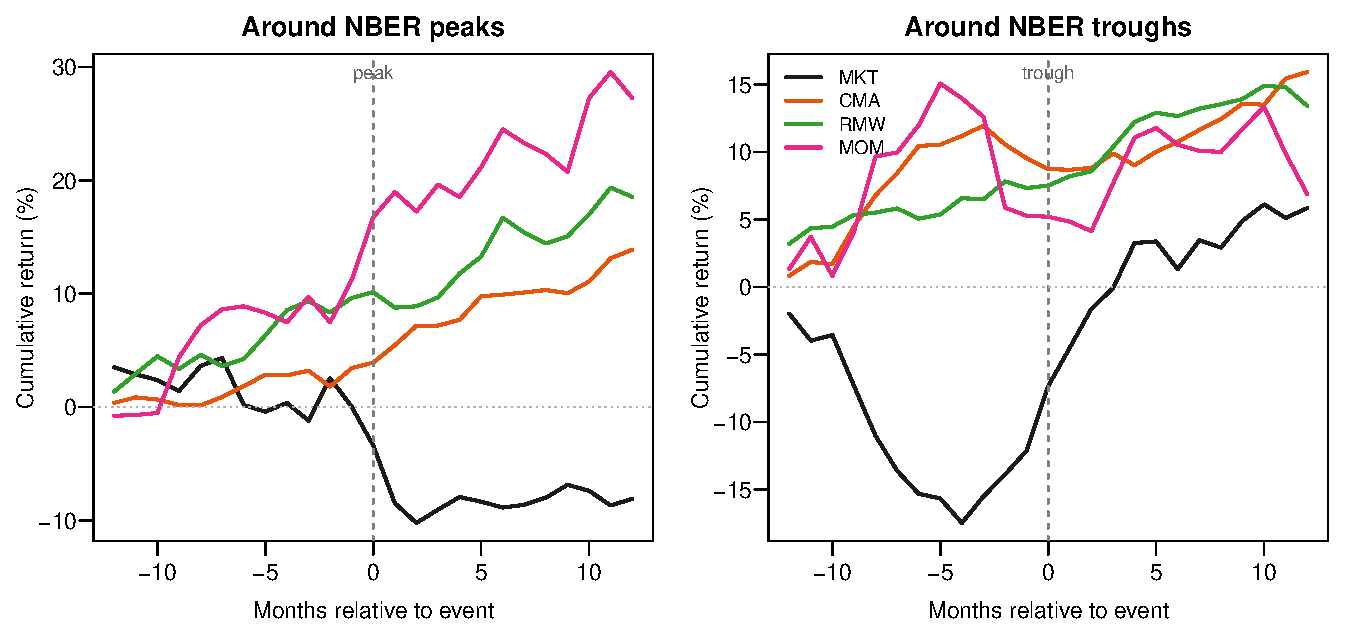
\includegraphics[width=\textwidth]{fig_event.pdf}
\caption{\textbf{Event-time cumulative factor returns around NBER peaks and
troughs.} Each line is the average cumulative return (\%) of a factor in event
time, accumulated from twelve months before the event and averaged across the
\nRecessions{} in-sample episodes. The vertical dashed line marks the
business-cycle turning point. Left: peaks. Right: troughs.}
\label{fig:event}
\end{figure}

% ===========================================================================
\section{Robustness: Subsample Stability}
\label{sec:robust}

Because recessions are infrequent, conditional means are estimated from a
limited number of months and could be driven by a single episode. As a check on
stability, Table~\ref{tab:subsample} re-estimates the recession-minus-expansion
differential separately in the first and second halves of the sample (split at
1990). The qualitative ordering is robust: the market's differential is large
and negative in both halves, and momentum's is negative in both. The
defensiveness of the quality factors is present in both subsamples but rotates
across them---CMA's positive differential is concentrated in the earlier period,
while RMW's is strongest after 1990---consistent with the two factors capturing
related but distinct facets of firm quality. Value's differential is positive
and significant before 1990 but turns negative afterward, which is why its
full-sample cyclicality washes out; this instability is itself a useful caution
against strong risk-based claims for HML over the modern sample.

We caution that the conditional differentials are estimated with limited
precision and that our classification is binary; richer conditioning on the
\emph{depth} of contractions, or on continuous macroeconomic state variables in
the spirit of \citet{lettau2001resurrecting} and \citet{henkel2011conditional},
is a natural extension. The robustness of the \emph{sign} pattern across
samples, across the NBER and real-time classifications, and in event time
nonetheless gives us confidence in the paper's qualitative conclusions.

\begin{table}[t]
\centering
\caption{\textbf{Subsample stability of the recession differential.} Annualized
recession-minus-expansion differential (\%) for each factor, estimated separately
over 1963--1989 and 1990--2026, with Newey--West $t$-statistics in parentheses.}
\label{tab:subsample}
\small
\begin{tabular}{lcccc}
\toprule
 & \multicolumn{2}{c}{1963--1989} & \multicolumn{2}{c}{1990--2026} \\
\cmidrule(lr){2-3}\cmidrule(lr){4-5}
Factor & Diff. & $t$ & Diff. & $t$ \\
\midrule
MKT & -11.18 & (-0.91) & -21.73 & (-1.37) \\
SMB & -4.30 & (-0.73) & 3.65 & (0.56) \\
HML & 8.37 & (1.44) & -12.05 & (-1.55) \\
RMW & -4.31 & (-1.20) & 8.73 & (1.84) \\
CMA & 13.87 & (2.69) & -3.34 & (-0.67) \\
MOM & -2.41 & (-0.34) & -16.24 & (-0.87) \\
\bottomrule
\end{tabular}

\end{table}

% ===========================================================================
\section{Conclusion}
\label{sec:conclusion}

We have asked whether the equity factors marketed as defensive actually deliver
when the economy contracts, and we find that the answer depends entirely on
which factor one means. The market and momentum are procyclical: they earn their
premia in good times and surrender them---momentum violently---in bad times. The
profitability and investment factors are genuinely defensive: their premia rise
in recessions, their Sharpe ratios peak in contractions, and they accumulate
returns steadily while the market falls into and climbs out of its troughs. Size
and value are acyclical, and value's lack of reliable procyclicality over the
modern sample sits awkwardly with risk-based interpretations. These conclusions
hold under the ex-post NBER dating, under a real-time tradeable signal, and in
event time.

The practical implication is that ``defensiveness'' is not a generic property of
factor investing but a specific property of factors built on firm
fundamentals---profitability and conservative investment---as opposed to those
built on prices and trends. For asset allocation, this suggests that quality
tilts can play the diversifying role often claimed for them, whereas momentum,
despite its high unconditional Sharpe ratio, concentrates its losses in exactly
the states where diversification is most valuable. For asset-pricing theory, the
heterogeneity we document is a reminder that a positive average premium is
consistent with very different conditional risk profiles, and that distinguishing
among the factors requires looking at when, not just whether, they pay.

\clearpage
\setstretch{1.1}
\bibliographystyle{plainnat}
\bibliography{references}

\end{document}
